\documentclass{article}
\usepackage[utf8]{inputenc}
\usepackage{graphicx}
\graphicspath{ {./images/} }
\usepackage{libertine}
\usepackage{libertinust1math}
\usepackage{float}

\title{Exercise 3 \\ Making, Analysing, Interpreting Observations}
\author{Maria Eirini Tzampazidou }
\date{September 2019}

\begin{document}

\maketitle

\section*{Introduction}

In the current report a Principal Component Analysis(PCA) takes place. The data used represent monthly sea surface height anomalies (1993-2018) with respect to a 20-year mean reference period (1993-2012), observed by a series of altimetry satellites. The original data come at a 0.25° resolution, and cover the global oceans, and were downloaded from: https://cds.climate.copernicus.eu/cdsapp#!/dataset/sea-level-daily-gridded-data-for-theglobal-ocean-from-1993-to-present?tab=overview .
In this exercises, we’ll focus on the tropical Pacific Ocean (here defined as 100° to 280°E; -29.75° to 29.75°N). The data has been downsampled to 0.5° resolution to reduce the file size and computational load.

\section*{Question 1}

\begin{figure}[b!]
\centering
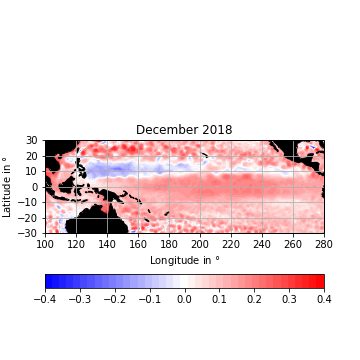
\includegraphics[width=1.0\linewidth]{December2018(initial).png}
\caption{Sea level anomaly December 2018}
\label{fig:DEC}
\end{figure}


Plotting a number of months can give a good overview of the data. December from year 2018 is a representative example of the phenomena taking place in the observed area. Knowing in advance that El nino periodically dominates this band of the Pacific ocean, we can easily interpret what is observed in Figure 1. Looking at the equator, the trend is generally positive.More specifically, the negative sea level anomaly(SLA) in the west between 3-15$^o$lat, 120-200$^o$ indicates 'the cold tongue' and the positive SLA between -3 - 10$^o$lat, 200-260$^o$ indicates the 'warm pool'. From 20$^o$-30$^o$ in both Northern and Southern Hemisphere we observe only positive SLA. Probably large scale gyres/eddies induce a positive sea surface elevation. 



\newpage
\section*{Question 2}
Now we apply the Empirical Orthogonal Function (EOF) analysis, sometimes also referred to as Principal Component Analysis (PCA). We start processing the data after forming the covariance matrix. Through this matrix we are able to derive eigenvectors and its eigenvalues. The eigenvectors represent the empirical orthogonal functions (i.e., spatial modes of variability), the eigenvalues give a measure of the total variance in the data explained. In other words, eigenvectors with a large eigenvalue explain more variability of the sea surface height anomalies than those with a small eigenvalue. How each EOF field evolves in time, can be found by projecting the eigenvector on the data matrix. This yields the principal component (PC) timeseries. After that we apply a normalisation to the EOFs and the PCs so that the absolute maximum value of each PC equals 1; since we scale the PC by a factor x(maximum PC value), the EOF needs to be scaled by 1/x. In Figure 2 and Figure 3 the EOFs and  PCs are shown respectively:

\begin{figure}[b!]
\centering
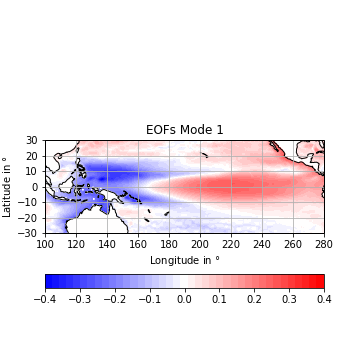
\includegraphics[width=1.0\linewidth]{EOFmode1.png}
\caption{EOF's for Mode 1}
\label{fig:EOF1}
\end{figure}

\begin{figure}[b!]
\centering
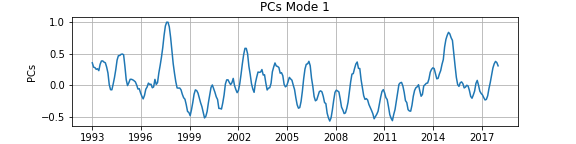
\includegraphics[width=1.0\linewidth]{PCsmode1.png}
\caption{PC's for Mode 1}
\label{fig:DPC1}
\end{figure}

Mode 1 in a PCA analysis explains the dominant pattern or trend of the data. The first principal component has the largest possible variance (that is, accounts for as much of the variability in the data as possible), and each succeeding component in turn has the highest variance possible under the constraint that it is orthogonal to the preceding components. 
After that, we can safely conclude that we are dealing with ENSO. In Figure 2 the cold tongue in the west and the warm pool in the east are even more pronounced since we only see the main pattern of SLA and not the background state. In Figure 3 we observe five high picks in band of 26 years, approximately every four-five years: 1997,2002,2006,2010,2014, and possibly at the end of 2018. According to the theory, this can be interpreted as the ENSO's period.



\section*{Question 3}
In order to fully inspect the data and interpret the results we perform a spectral analysis of each mode. We first apply a Fourier transformation of our signal (PCs) and then we calculate the spectral power according to equation 1:
\begin{equation}
    SpectrumPower = |FourierTransformation|^2
\end{equation}

Now, we are looking at Modes 2 and 3 through Figures 4 and 7 for the EOF's and through Figures 5 and 8 for the PC's. We already expect less variability; their trends are not so pronounced, and their cycle probably repeated more often; they have smaller periods. This is exactly what we observe in the associated Figures. In the same time mode 2 is negative in NH winter and positive in NH summer and mode 3 is positive in NH spring and negative in NH autumn.
\\Looking at Figures 6 and 9 we can see the corresponding spectral power. Looking at the spectral power we can precisely determine the cycles of repeated phenomena. Looking at the spectra for mode 2 and 3 we observe a peak every one year. So in our case, modes 2 and 3 express seasonal small scale trends. However, this is not the case if we plot the spectral power of mode 1.If we look at Figure 10, we observe one not so clear spectrum. The highest peak corresponds to a frequency of 0.000620347 per day. If we convert it to years, and then calculate the period it corresponds to a cycle of 4.14. This number confirms the periodic peaks in the eigenvalues plot. 
\\We conclude that our approximation about ENSO according to the SLA is confirmed once more. 
\begin{figure}[b!]
\centering
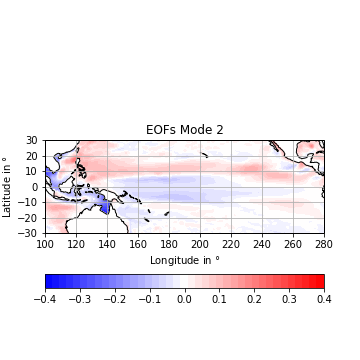
\includegraphics[width=1.0\linewidth]{EOFmode2.png}
\caption{EOF's for Mode 2}
\label{fig:EOF2}
\end{figure}

\begin{figure}[b!]
\centering
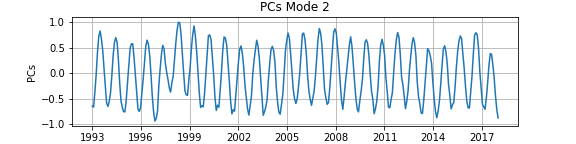
\includegraphics[width=1.0\linewidth]{PCsmode2.png}
\caption{PC's for Mode 2}
\label{fig:PC2}
\end{figure}

\begin{figure}[b!]
\centering
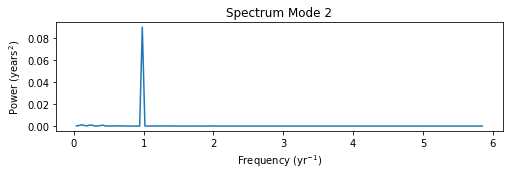
\includegraphics[width=1.0\linewidth]{Spectrum2.png}
\caption{Spectral Power for Mode 2}
\label{fig:PC2}
\end{figure}

\begin{figure}[b!]
\centering
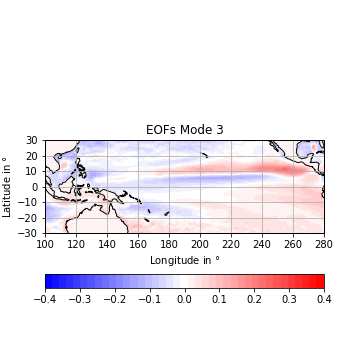
\includegraphics[width=1.0\linewidth]{EOFmode3.png}
\caption{EOF's for Mode 3}
\label{fig:EOF3}
\end{figure}

\begin{figure}[b!]
\centering
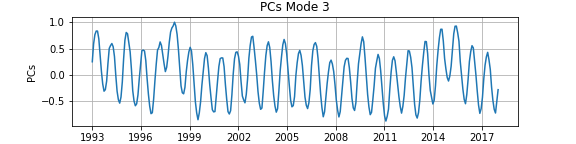
\includegraphics[width=1.0\linewidth]{PCsmode3.png}
\caption{PC's for Mode 3}
\label{fig:PC3}
\end{figure}

\begin{figure}[b!]
\centering
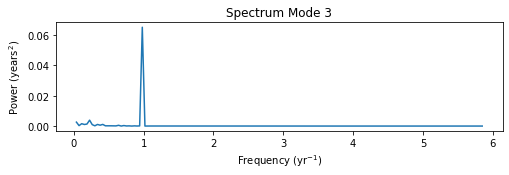
\includegraphics[width=1.0\linewidth]{spectrum3.png}
\caption{Spectral Power for Mode 3}
\label{fig:PC2}
\end{figure}

\begin{figure}[b!]
\centering
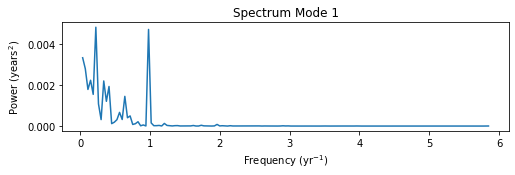
\includegraphics[width=1.0\linewidth]{spectrum1.png}
\caption{Spectral Power for Mode 1}
\label{fig:spec1}
\end{figure}

\section*{Question 4}
As it has been already mentioned the first mode explains the largest variability compared to the rest while mode 2 and 3 show seasonal trends.
In this section a representation of the cumulative fraction of explained variance of all modes is given through Figure 11. The curve indicates the excess of the first modes, and especially Mode 1. All the modes are 312, as our time spots. Each time spot represents a month. 

\section*{Question 5}
In the end we are interested to see how good the data will be represented according to the information from the first six modes only. The total variance contained in this reconstructed data is the one from the modes 1-6. We can observe the results for December 2018 in Figure 12: We can clearly identify the main patterns(cold tongue, warm pool). However the smaller SLA are not so clear; the positive SLA background in the band of 20-30$^o$ North and South are not identified, especially in the Southern Hemisphere. In order to increase the amount of information we can get we should plot more modes. If we now look at the differences between the initial data about December 2018 and the reconstructed we can see that modes 1-6 do not give a sufficient representation indeed. 
\begin{figure}[b!]
\centering
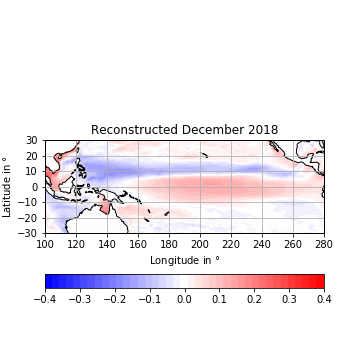
\includegraphics[width=1.0\linewidth]{reconstructedDec.png}
\caption{Reconstructed data for December 2018.}
\label{fig:recDEC}
\end{figure}

\begin{figure}[b!]
\centering
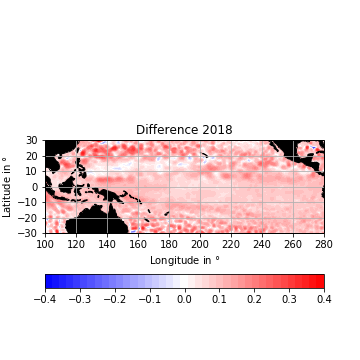
\includegraphics[width=1.0\linewidth]{difference.png}
\caption{Difference between initial and reconstructed data for December 2018. }
\label{fig:diff}
\end{figure}


\end{document}
